\section{フロベニウスと共に類体論の碧落へ}\label{hekiraku}
\subsection{使うためのガロア理論と円分体}
\textbf{群論を眼下にトラバース------。}

\vspace{10pt}

\textbf{代数体$L,K$に対して}$L/K$が体の有限次拡大である時,必ず\[
L=K(\alpha)=\left\{\frac{g(\alpha)}{f(\alpha)}\mid f(x),g(x)\in K[x],\; f(\alpha)\ne 0\right\}
\]となる$\alpha\in L$が存在することが知られている。
\begin{dfn}[ガロア拡大,ガロア群]
    代数体の有限次拡大$L/K$に対し,$L=K(\alpha)$を満たす$\alpha\in L$をとる。$\alpha$の$K$上の最小多項式$\phi_{\alpha}(x)$のすべての根$\alpha=\alpha^{(1)},\alpha^{(2)},\ldots,\alpha^{(n)}$が$L$の元となる時,$L/K$は\textbf{ガロア拡大}であるという.ガロア拡大$L/K$において,$K$への制限が恒等写像で,$L$上の体自己同型であるもの全体の集合を$\boldsymbol{\textrm{Gal}(L/K)}$と書き,$L/K$の\textbf{ガロア群}と呼ぶ.
\end{dfn}

定義から直ちにわかる,次のことを確認しよう:
\begin{itemize}
    \item $[L:K]=\#\textrm{Gal}(L/K).$
    \item ガロア群の元は,$\phi_{\alpha}(x)$の根の置換を引き起こす写像である。
    \item $\mathbb{Q}(\sqrt[3]{2})/{\mathbb{Q}}$はガロア拡大ではない代数体の有限次拡大である(証明しよう)。
\end{itemize}

\begin{dfn}[中間体]
    $L/K$を体の拡大とする.部分体$M\subset L$で$K$を含むものを$L/K$の\textbf{中間体}という.
\end{dfn}

ガロア理論の中核である\textbf{ガロアの基本定理}の(ガロア拡大$L/K$についての)主張は概ね次の通りである:
\begin{quote}
    $\textrm{Gal}(L/K)$の部分群$H$に対して,\textbf{$H$の不変体}$L_H\coloneqq\left\{x\in L\mid\forall g\in H,\, g(x)=x\right\}$が対応する.特に,$L/K$の中間体と$\mathrm{Gal}(L/K)$の部分群は1対1に対応する。
\end{quote}

\vspace{15pt}

\begin{dfn}[円分体]
    $\zeta_n\coloneqq e^{\frac{2\pi\sqrt{-1}}{n}}$を1の原始$n$乗根とする.$\mathbb{Q}$に$\zeta_n$を添加した$\mathbb{Q}(\zeta_n)$を\textbf{($n$次)円分体}という.
\end{dfn}
\begin{dfn}[オイラー関数]
    $(\mathbb{Z}/{n\mathbb{Z}})^{\times}$を$\mathbb{Z}/{n\mathbb{Z}}$の乗法群($n$と互いに素な整数$a$の剰余類を集めたもの)とする.$\varphi:\mathbb{Z}^+\ni n\mapsto\# (\mathbb{Z}/{n\mathbb{Z}})^{\times}\in\mathbb{Z}^+$を\textbf{オイラー関数}と呼び,必ず$\varphi$で表すことにする.
\end{dfn}
\begin{dfn}[円分多項式]
    $\varphi(n)$次多項式\[
    \Phi_n(x)=\prod_{k+n\mathbb{Z}\in(\mathbb{Z}/{n\mathbb{Z}})^{\times}}(x-\zeta_n^k)
    \]は$\mathbb{Z}$上既約な$\mathbb{Z}[x]$の元であるが,これを\textbf{円分多項式}と呼ぶ.
\end{dfn}
円分多項式は,$\mathbb{Z}$上の最小多項式となることが知られている。したがって,$\Phi_n(x)=\phi_{\zeta_n}(x)$である。また,$\mathcal{O}_{\mathbb{Q}(\zeta)}=\mathbb{Z}[\zeta]$も成り立つ。

なぜ円分体なるものを定義するのだろうか?モチベーションを得るために紹介する事柄がある:
\begin{mybox}[ガウス和]
    $\mathbb{Q}(\sqrt{-1})=\mathbb{Q}(\zeta_4)$より,$\mathbb{Q}(\sqrt{-1})$は4次円分体である。実は,例えば$\mathbb{Q}(\sqrt{-7})$のように円分体でないものも,円分体との関係がある:$\sqrt{-7}=(\zeta_7+\zeta_7^2+\zeta_7^4)-(\zeta_7^3+\zeta_7^5+\zeta_7^6)$という等式があり,$\mathbb{Q}(\sqrt{-7})\subset\mathbb{Q}(\zeta_7)$となるのだ。このように,奇素数$p$に対して\[
    G_p\coloneqq\sum_{i=1}^{p-1}\left(\frac{k}{p}\right)e^{\frac{2\pi\sqrt{-1}}{p}i}
    \]と定義される$G_p$を\textbf{ガウス和}という。ガウス和について,一般にも次のことが成り立つ(!):\[
    G_p=\begin{cases*}
        \sqrt{p}&($p\equiv 1\pmod{4}$)\\
        \sqrt{-p}&(otherwise)
    \end{cases*}
    \]今まで扱ってきた平方根を添加した体と円分体には関係があることがわかった。
\end{mybox}
\begin{mybox}[フェルマー予想(テイラー-ワイルスの定理)]
    1823年のMarie-Sophie Germainによる結果など,フェルマー予想の個別でないケースについての結果はあったが,「クンマーの定理」として知られる正則素数全体についてのフェルマー予想の解決には,円分体の整数環による考察が必要であった。
\end{mybox}
他にもモチベーションになり得る事柄は数多あるが,先を急ごう。$\mathbb{Q}(\zeta_n)/{\mathbb{Q}}$を\textbf{円分拡大}という。円分拡大について少し見ておこう:

まず,定義からわかるように,$\zeta_n$の最小多項式である円分多項式$\Phi_n(x)$は,$\zeta_n^k\,(k\text{と}n\text{は互いに素})$を根に持つ。$\mathbb{Q}(\zeta_n)/{\mathbb{Q}}$はガロア拡大となり,$\#\mathrm{Gal}(\mathbb{Q}(\zeta_n)/{\mathbb{Q}})=\varphi(n)$となる。ここで,$\sigma_k:\zeta_n\mapsto\zeta_n^k\, (k\in (\mathbb{Z}/{n\mathbb{Z}})^{\times})$を考えると,$(\mathbb{Z}/{n\mathbb{Z}})^{\times}\ni k+n\mathbb{Z}\mapsto\sigma_k\in\mathrm{Gal}(\mathbb{Q}(\zeta_n)/{\mathbb{Q}})$は群同型である。ここで,ガロアの基本定理から$\mathbb{Q}(\zeta_n)$の部分体は,$\mathrm{Gal}(\mathbb{Q}(\zeta_n)/{\mathbb{Q}})$の部分群$H$の不変体$\mathbb{Q}(\zeta_n)_H=\{x\in\mathbb{Q}(\zeta_n)\mid\forall g\in H,\, g(x)=x\}$として与えられる。難しく思われる「中間体を求める」というタスクを,「群の構造を調べる」比較的容易な作業に落とし込めるのが,ガロア理論の強さである。

\subsection{有限体のガロア理論}
\textbf{山頂付近の空が晴れてきた------。}

\vspace{10pt}

ここで準備として有限体,つまり位数が有限の体,の拡大のガロア群を考えよう。まずは,有限体の基本的な性質を挙げる:
\begin{itemize}
    \item 位数の等しい有限体はすべて同型で,任意の有限体はある素数$p$に対する$\mathbb{F}_{p^n}$($n$はその有限体の位数に等しい)と同型である。
    \item $q,q'$を素数のべき乗とする。$\mathbb{F}_{q'}$が$\mathbb{F}_{q}$の拡大体となるのは,$q'$が$q$で割り切れる時,かつその時に限り,体の拡大$\mathbb{F}_{q'}/{\mathbb{F}_q}$はガロア拡大である。
\end{itemize}
ここで,久しぶりにフロベニウスが登場する\dots\dots というか,フロベニウスが待ってくれていたのだ。ただいま:

$q,q'$を素数$p$のべき乗とし,$q\mid q'$とすると,ガロア拡大$\mathbb{F}_{q'}/{\mathbb{F}_q}$のガロア群$\mathrm{Gal}(\mathbb{F}_{q'}/{\mathbb{F}_q})$は,\textbf{フロベニウス自己同型}$\mathrm{Frob}_q:\mathbb{F}_{q'}\ni x\mapsto x^q\in\mathbb{F}_{q'}$が生成する巡回群$\langle\mathrm{Frob}_q\rangle$となることが知られている。ここで有限体のガロア群の生成元として表れたフロベニウスは,より一般の拡大について考える際にも登場する。

\subsection{代数体の一般化に向けて}\label{ippanka}
\textbf{もう雲を抜けたんだ------。}

\vspace{10pt}

一般の代数体$K$の整数環$\mathcal{O}_K$は,今までの議論で扱ってきたものより複雑になり得ることは想像に難くない。素数が生成する単項イデアルによって,素数の分解について考えるだけでは済まない。そこで,「素数を分解する」世界を抜けて,「素イデアルを分解する」世界に入ろう。

代数体の有限次拡大$L/K$を考える。整数環$\mathcal{O}_K$の素イデアル$\mathfrak{p}$が,1つ``上''の$\mathcal{O}_L$でどのように分解するか,調べたい。$\mathcal{O}_L$上でも$\mathfrak{p}$を扱うために,$\mathfrak{p}$が生成する$\mathcal{O}_L$のイデアル$\mathfrak{p}\mathcal{O}_L$を考える。素イデアル分解の一意性より,
\begin{equation}\label{prime_bunkai}
\mathfrak{p}\mathcal{O}_L=\mathfrak{P}_1^{e_1}\mathfrak{P}_2^{e_2}\cdots\mathfrak{P}_g^{e_g}\; (\mathfrak{P}_1,\ldots,\mathfrak{P}_g\text{は相異なる}\mathcal{O}_L\text{の素イデアル})
\end{equation}
と書ける(ちなみに,ごつい文字$\mathfrak{P}$は,フラクトゥーアにおける大文字の「\ruby{P}{ペー}」)。ここで,イデアルの積の定義より,$\mathfrak{P}_i\supset\mathfrak{P}_1^{e_1}\cdots\mathfrak{P}_g^{e_g}=\mathfrak{p}\mathcal{O}_L\supset\mathfrak{p}$であるが,これを$\mathfrak{P}_i\mid\mathfrak{p}$で表現する。また,$\mathfrak{P}_i\cap\mathcal{O}_K=\mathfrak{p}$であることもわかる(後で使う)\footnote{ホントはこれを示すには,極大イデアルというものを知っている必要がある。下の方で有限体$\mathcal{O}_K/{\mathfrak{p}}$が出てくるが,これが有限体であることも,極大イデアルを知らなければ示せない。}。

\begin{dfn}[分解指数,分岐指数]
    上記の$\mathfrak{p}\mathcal{O}_L$の素イデアル分解の下で,$g$を$\mathfrak{p}$の\textbf{分解指数}と呼ぶ.また,$e_i$を,$\mathfrak{P}_i$の$L/K$における\textbf{分岐指数}と呼び,$e_i=1$なら,$\mathfrak{P}_i$は$L/K$で不分岐であるという.
\end{dfn}

ここで,有限体$\mathcal{O}_K/{\mathfrak{p}},\,\mathcal{O}_L/{\mathfrak{P}_i}$について,$\mathcal{O}_L/{\mathfrak{P}_i}$は$\mathcal{O}_K/{\mathfrak{p}}$の有限次拡大体である。
\begin{dfn}[惰性次数]
    上記の下,$f_i\coloneqq [\mathcal{O}_L/{\mathfrak{P}_i}:\mathcal{O}_K/{\mathfrak{p}}]$とし,$f_i$を,$\mathfrak{P}_i$の$L/K$における\textbf{惰性次数}と呼ぶ.
\end{dfn}
惰性次数の定義の方は,何がしたいのかわからないと思うが,次の定理がある:
\begin{thm}\label{toshiki_sp}
    \[
    [L/K]=\sum_{i=1}^{g}e_if_i
    \]が成り立つ.
\end{thm}
この定理はCRTから導かれる同型$\mathcal{O}_L/{\mathfrak{p}\mathcal{O}_L}\cong\prod_{i=1}^{g}\mathcal{O}_L/{\mathfrak{P}_i^{e_i}}$を用いて,次元に注目すれば示せる(証明は簡単ではないが省略)。

上記定理を用いると,「完全分解」など聞き覚えのある言葉を定義できる。この定義と先の定理を合わせれば惰性次数の意義が掴める:
\begin{dfn}[聞き覚えのある用語+「分岐」]
    \begin{itemize}
        \item $e_1,\ldots,e_g$の少なくとも1つが1より大きい時,$\mathfrak{p}$は$L$で\textbf{分岐する},という.
        \item $e_i$がすべて1である時,$\mathfrak{p}$は$L$で\textbf{不分岐する},という.
        \item $e_1=n$,つまり$g=f_i=1$の時,$\mathfrak{p}$は$L$で\textbf{完全分岐する},という.
        \item 不分岐かつ,$f_i$がすべて1である時,$\mathfrak{p}$は$L$で\textbf{完全分解する},という.
        \item 不分岐かつ,惰性次数が$[L:K]$に等しい時,$\mathfrak{p}$は$L$で\textbf{惰性する},という.
    \end{itemize}
\end{dfn}
平方根を添加した世界で考えた際もそうだったが,分岐するケースは特殊であるため,以降は,不分岐の場合を主として扱うことになる。

まず,$\mathfrak{p}$が完全分岐するとき,$\mathfrak{p}=\mathfrak{P}^{n}(\mathfrak{P}\text{は素イデアル})$というふうになる。$\mathfrak{p}$が完全分解する時,定理\ref{toshiki_sp}より,$g=[L:K]$となり,$\mathfrak{p}$は可能な限り最も多くの相異なる素イデアルに分解することになる。$\mathfrak{p}$が惰性する時は,再び定理\ref{toshiki_sp}より,$g=1$となり,分解しないで素イデアルのままとなる。これが,惰性次数が惰性の次数たるゆえんである。

\subsection{ガロア拡大におけるヒルベルトの分岐理論}
\textbf{代数体と有限体の吊尾根を往く------。}

\vspace{10pt}

ここでは,素イデアルの分解を説明する「ヒルベルト理論」を紹介する。前の\ref{ippanka}項で使った記号は断りなくそのまま使う(分岐指数$e_i$とか惰性次数$f_i$とか)。また,$L/K$をガロア拡大とし,$G\coloneqq\mathrm{Gal}(L/K)$とする。さらに,$n\coloneqq [L/K]$とおく。

$\mathfrak{p}\mathcal{O}_L$の素イデアル分解\eqref{prime_bunkai}を思い出そう。任意の$\sigma\in G$に対し,$\sigma(\mathfrak{P}_i)$は素イデアルとなる(示してみよう)が,ガロア群の定義より$\sigma$の$K$への制限は恒等写像であり,$\mathfrak{P}_i\cap\mathcal{O}_K=\mathfrak{p}$であったから,\[
\sigma(\mathfrak{P}_i)\cap\mathcal{O}_K=\sigma(\mathfrak{P}_i\cap\mathcal{O}_K)=\sigma(\mathfrak{p})=\mathfrak{p}
\]となり,$\exists j,\,\sigma(\mathfrak{P}_i)=\mathfrak{P}_j$である。さらに,ある1つの$\mathfrak{P}_i$に対し,$G$のすべての元を作用させると,$\mathfrak{P}\mid\mathfrak{p}$を満たすすべての$\mathfrak{P}$(つまり,$\mathfrak{p}\mathcal{O}_L$のすべての``素因数'')に移れることが示せる。

ここで,$\mathfrak{p}\mathcal{O}_L$の素イデアル分解\eqref{prime_bunkai}の両辺に$\sigma\in G$を作用させることを考える。すると,$\mathfrak{p}\subset K$より$\sigma(\mathfrak{p}\mathcal{O}_L)=\mathfrak{p}\mathcal{O}_L$であるから,$\exists j,\, \sigma(\mathfrak{P}_i)=\mathfrak{P}_j$より$\sigma(\mathfrak{P}_i^{e_i})=\mathfrak{P}_j^{e_i}$となって素イデアル分解の一意性から$\mathfrak{P}_j^{e_i}=\mathfrak{P}_j^{e_j}$となる。したがって,すべての$i$にわたって分岐指数は等しくなる:$e_1=\cdots=e_g$.これを$e$とおく。さらに,惰性次数もすべて等しいことが示せるから,これを$f$とおく。

よって,定理\ref{toshiki_sp}の主張は
\begin{equation}\label{toshiki_sp_galois}
n=[L/K]=efg
\end{equation}と単純になり,これがガロア拡大を考えるモチベーションになる。

ここで再び$\sigma\in G$を$\mathfrak{P}_i$に作用させることを考える。以下,$\mathfrak{P}\mid\mathfrak{p}$を1つ取って考える。特に,不動点に注目しよう:
\begin{dfn}[分解群,分解体]
    \[
    Z_{\mathfrak{P}}\coloneq\left\{\sigma\in G\mid\sigma(\mathfrak{P})=\mathfrak{P}\right\}
    \]とすると,これは$G$の部分群であり,$L/K$における$\mathfrak{P}$の\textbf{分解群}という.また,$Z_{\mathfrak{P}}$の不変体$L_{Z_{\mathfrak{P}}}$(ガロアの基本定理により$Z_{\mathfrak{P}}$と対応する中間体)を\textbf{分解体}という.
\end{dfn}
分解群の元によって$\mathfrak{P}$は動かないから,$Z_{\mathfrak{P}}$の後に$\sigma\in G$を作用させた$\sigma Z_{\mathfrak{P}}$は,$\mathfrak{P}$を$\mathfrak{P'}\mid\mathfrak{p}$なる異なる$\mathfrak{P'}$に移す。したがって,$G/{Z_{\mathfrak{P}}}=\{\sigma_1Z_{\mathfrak{P}},\ldots,\sigma_gZ_{\mathfrak{P}}\}$の各元は,$\mathfrak{P}$を相異なる素イデアル$\mathfrak{P}_1,\ldots,\mathfrak{P}_g$に移し,
\begin{equation}\label{zentan_zp}
G/{Z_{\mathfrak{P}}}\rightarrow\{\mathfrak{P}_1,\ldots,\mathfrak{P}_g\}
\end{equation}
は全単射である。よって,$\# (G/Z_{\mathfrak{P}})=g$である。分解群は分解の仕方を反映しているのだ。

さらに,$n=\# G$に注目しよう。すると,ガロアの基本定理の証明にも使われる「アルティンの定理」というものにより,
\begin{equation}\label{dokei_galois_artin}
\mathrm{Gal}(Z_{\mathfrak{P}}/{L_{Z_{\mathfrak{P}}}})\cong Z_{\mathfrak{P}}
\end{equation}
が成り立つから,ガロアの基本定理で与えられる対応は$\mathrm{Gal}(L/\cdot)$という操作にあたることがわかる。したがって,$\# Z_{\mathfrak{P}}=ef$となり,対応関係を表現した図\ref{fig:tikz_field}の一部がわかる。

\begin{figure}[ht]
    \centering
    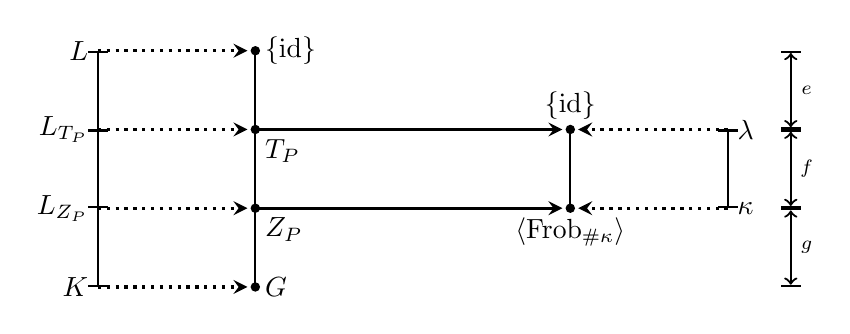
\begin{tikzpicture}
        \coordinate[label=left:$L$] (L) at (-1,1.5);
        \coordinate[label=left:$L_{T_{\mathfrak{P}}}$] (M) at (-1,0.5);
        \coordinate[label=left:$L_{Z_{\mathfrak{P}}}$] (N) at (-1,-0.5);
        \coordinate[label=left:$K$] (K) at (-1,-1.5);
        \coordinate[label=right:$\{\textrm{id}\}$] (id) at (1,1.5);
        \coordinate[label=below right:$T_{\mathfrak{P}}$] (T) at (1,0.5);
        \coordinate[label=below right:$Z_{\mathfrak{P}}$] (Z) at (1,-0.5);
        \coordinate[label=right:$G$] (G) at (1,-1.5);
        \draw[thick] (id)--(G);
        \draw[|-|,thick] (L)--(K);
        \draw[|-|,thick] (M)--(N);
        \draw[->,dotted,very thick,>=stealth] (L)--(0.9,1.5);
        \draw[->,dotted,very thick,>=stealth] (M)--(0.9,0.5);
        \draw[->,dotted,very thick,>=stealth] (N)--(0.9,-0.5);
        \draw[->,dotted,very thick,>=stealth] (K)--(0.9,-1.5);
        \draw[->,very thick,>=stealth] (T)--(4.9,0.5);
        \draw[->,very thick,>=stealth] (Z)--(4.9,-0.5);
        \coordinate[label=above:$\{\mathrm{id}\}$] (id_a) at (5,0.5);
        \coordinate[label=below:$\boldsymbol{\langle\mathrm{Frob}_{\#\kappa}\rangle}$] (frob) at (5,-0.5);
        \draw[thick] (id_a)--(frob);
        \coordinate[label=right:$\lambda$] (lambda) at (7,0.5);
        \coordinate[label=right:$\kappa$] (kappa) at (7,-0.5);
        \draw[|-|,thick] (lambda)--(kappa);
        \draw[->,dotted,very thick,>=stealth] (lambda)--(5.1,0.5);
        \draw[->,dotted,very thick,>=stealth] (kappa)--(5.1,-0.5);
        \fill (id) circle [radius=0.06];
        \fill (T) circle [radius=0.06];
        \fill (Z) circle [radius=0.06];
        \fill (G) circle [radius=0.06];
        \fill (id_a) circle [radius=0.06];
        \fill (frob) circle [radius=0.06];
        \node at (8,1) {\scriptsize$e$};
        \node at (8,0) {\scriptsize$f$};
        \node at (8,-1) {\scriptsize$g$};
        \draw[|<->|,thick] (7.8,0.5)--(7.8,1.5);
        \draw[|<->|,thick] (7.8,-0.5)--(7.8,0.5);
        \draw[|<->|,thick] (7.8,-1.5)--(7.8,-0.5);
    \end{tikzpicture}
    \caption{ヒルベルト理論の対応関係}\label{fig:tikz_field}
\end{figure}

次に,「惰性群」というものを定義する。以降,$\lambda\coloneq\mathcal{O}_L/{\mathfrak{P}},\,\kappa\coloneq\mathcal{O}_K/{\mathfrak{p}}$とする。$x+\mathfrak{P}\in\lambda$と$\sigma\in Z_{\mathfrak{P}}$に対して,$\sigma(x+\mathfrak{P})=\sigma(x)+\mathfrak{P}$となることから,$\sigma$は$\lambda$の自己同型となり,$\sigma$は$\mathcal{O}_K$の元を固定するため$\kappa$の元も固定する。したがって,$\sigma$は$\mathrm{Gal}(\lambda/{\kappa})$の元$\bar{\sigma}$を定め,対応\[
\pi:Z_{\mathfrak{P}}\ni\sigma\mapsto\bar{\sigma}\in\mathrm{Gal}(\lambda/\kappa)
\]が誘導される。$\pi$は単射でない全射準同型となる。そこで,単射にして同型をつくるために,次の群を定義する:
\begin{dfn}[惰性群,惰性体]
    \[
    T_{\mathfrak{P}}\coloneqq\{\sigma\in Z_{\mathfrak{P}}\mid\forall x\in\mathcal{O}_L,\,\sigma(x+\mathfrak{P})=x+\mathfrak{P}\}
    \]とし,$T_{\mathfrak{P}}$を$L/K$における$\mathfrak{P}$の\textbf{惰性群}という.また,$T_{\mathfrak{P}}$の不変体$L_{T_{\mathfrak{P}}}$(ガロアの基本定理により$T_{\mathfrak{P}}$と対応する中間体)を\textbf{惰性体}という.
\end{dfn}
定義から$T_{\mathfrak{P}}=\mathrm{Ker}(\pi)$であるから,群の第一同型定理より,$T_{\mathfrak{P}}$のおかげで$Z_{\mathfrak{P}}/{T_{\mathfrak{P}}}\cong\mathrm{Gal}(\lambda/\kappa)$という同型が得られる。ここで,有限体のガロア理論を思い出すと,$\mathrm{Gal}(\lambda/\kappa)=\langle\mathrm{Frob}_{\#\kappa}\rangle$がわかる(フロベニウス!)。また,$Z_{\mathfrak{P}}$,$Z_{\mathfrak{P}}/{T_{\mathfrak{P}}}$の位数はそれぞれ$ef$,$f$だから,$\# T_{\mathfrak{P}}=e$である。以上で,図\ref{fig:tikz_field}の対応関係が明らかになった。

続いて,体の拡大に対応してどのように素イデアル$\mathfrak{p}$が分解されていくかを見る(おまけ)。$D_{\mathfrak{P}}\coloneqq L_{Z_{\mathfrak{P}}},\; I_{\mathfrak{P}}\coloneqq L_{T_{\mathfrak{P}}}$とする。

まず,$\mathfrak{P}_D\coloneqq\mathfrak{P}\cap\mathcal{O}_{D_{\mathfrak{P}}}$とおくと,$\mathfrak{P}_D\mid\mathfrak{P}$となる。さらに,$\mathfrak{P}_D$の$D_{\mathfrak{P}}/K$における分岐指数,惰性次数を$e',\; f'$とする。同型\eqref{dokei_galois_artin}より,$\mathrm{Gal}(L/D_{\mathfrak{P}})\cong Z_{\mathfrak{P}}$だが,$G$に$\mathrm{Gal}(L/D_{\mathfrak{P}})\cong Z_{\mathfrak{P}}$を当てはめて全単射\eqref{zentan_zp}を考えると,全単射$Z_{\mathfrak{P}}/Z_\mathfrak{P}\rightarrow\{\mathfrak{P}_{D,1},\ldots,\mathfrak{P}_{D,g'}\}$\; ($\{\mathfrak{P}_{D,1},\ldots,\mathfrak{P}_{D,g'}\}$は$\mathfrak{P'}\mid\mathfrak{P}_D$をみたす$\mathcal{O}_L$の素イデアル$\mathfrak{P'}$全体)が得られ,$g'=1$となる。$\mathfrak{P}_D$の$L/{D_{\mathfrak{P}}}$における分岐指数,惰性次数,分解指数はそれぞれ$e/e',\; f/f',\; g'=1$となるから,等式\eqref{toshiki_sp_galois}より,$[L:D_{\mathfrak{P}}]=\frac{e}{e'}\times\frac{f}{f'}\times 1$である。同時に,$[L:D_{\mathfrak{P}}]=\#\mathrm{Gal}(L/D_{\mathfrak{P}})=\# Z_{\mathfrak{P}}=ef$であるから,$e'=f'=1$である。したがって,すべての$\mathfrak{P}_D\mid\mathfrak{p}$の$D_{\mathfrak{P}}/K$における分岐指数と惰性次数が1となり,$\mathfrak{p}$は$D_{\mathfrak{P}}/K$で完全分解する。

次に,$\mathfrak{P}_I\coloneqq\mathfrak{P}\cap\mathcal{O}_{I_{\mathfrak{P}}}$とおく。すると,詳細は省略するが,$\mathcal{O}_{I_{\mathfrak{P}}}/\mathfrak{P}_I=\mathcal{O}_L/\mathfrak{P}$が示せる。したがって,$\mathfrak{P}_I$の$I_{\mathfrak{P}}/D_{\mathfrak{P}}$における惰性次数が$f$であり,等式\eqref{toshiki_sp_galois}と$[I_{\mathfrak{P}}:D_{\mathfrak{P}}]=\# (Z_{\mathfrak{P}}/T_{\mathfrak{P}})=f$より分岐指数が1であることがわかるので,$\mathfrak{P}_D$は$I_{\mathfrak{P}}/D_{\mathfrak{P}}$で惰性する。さらに,等式\eqref{toshiki_sp_galois}から,$\mathfrak{P}_I$が$L/I_\mathfrak{P}$で完全分岐することもわかり,図\ref{fig:tikz_bunkai_p}のようになる。ガロア拡大における素イデアルの分解が具にわかってしまった。
\begin{figure}[ht]
    \centering
    \begin{tikzpicture}
        \coordinate[label=left:$L$] (L) at (-1,1.5);
        \coordinate[label=left:$I_{\mathfrak{P}}$] (M) at (-1,0.5);
        \coordinate[label=left:$D_{\mathfrak{P}}$] (N) at (-1,-0.5);
        \coordinate[label=left:$K$] (K) at (-1,-1.5);
        \draw[|-|,thick] (L)--(K);
        \draw[|-|,thick] (M)--(N);
        \node at (1.2,1) {\scriptsize$e$};
        \node at (1.2,0) {\scriptsize$f$};
        \node at (1.2,-1) {\scriptsize$g$};
        \draw[|->|,>=stealth,thick] (1,0.5)--(1,1.5);
        \draw[|->|,>=stealth,thick] (1,-0.5)--(1,0.5);
        \draw[|->|,>=stealth,thick] (1,-1.5)--(1,-0.5);
        \node[below] at (1,-1.5) {$\mathfrak{p}$};
        \node[right] at (1.2,-0.5) {$\mathfrak{p}\mathcal{O}_{D_{\mathfrak{P}}}=\mathfrak{P}_1'\cdots\mathfrak{P}_g'\, (\mathfrak{P}_1'=\mathfrak{P}_D)$,$\mathfrak{p}$は完全分解};
        \node[right] at (1.2,0.5) {$\mathfrak{P}_D\mathcal{O}_{I_{\mathfrak{P}}}=\mathfrak{P}_I$,$\mathfrak{P}_D$は惰性};
        \node[right] at (1.2,1.5) {$\mathfrak{P}_I\mathcal{O}_L=\mathfrak{P}^e$,$\mathfrak{P}_I$は完全分岐};
        \draw[dotted,thick] (L)--(1,1.5);
        \draw[dotted,thick] (M)--(1,0.5);
        \draw[dotted,thick] (N)--(1,-0.5);
        \draw[dotted,thick] (K)--(1,-1.5);
    \end{tikzpicture}
    \caption{$\mathfrak{p}$の分解のしかた}\label{fig:tikz_bunkai_p}
\end{figure}

\subsection{フロベニウスとともに頂へ}
\textbf{類体論縦走------。}

\vspace{10pt}

この節では,類体論においてフロベニウスがどのように活躍しているかを見る。以下,$\mathfrak{p}$は不分岐とする。

先ほどのヒルベルト理論の帰結として,$Z_{\mathfrak{P}}\cong\mathrm{Gal}(\lambda/\kappa)=\langle\mathrm{Frab}_{\#\kappa}\rangle$が得られた。分解のしかたに関わる分解群を,フロベニウスを通して調べられる,ということだ。
\begin{dfn}[フロベニウス元]
    同型$Z_{\mathfrak{P}}\cong\langle\mathrm{Frab}_{\#\kappa}\rangle$によって$\mathrm{Frob_{\#\kappa}}$と対応する$Z_{\mathfrak{P}}$の生成元を$\left[\frac{L/K}{\mathfrak{P}}\right]$とかき,$L/K$における$Z_{\mathfrak{P}}$の\textbf{フロベニウス元}という.
\end{dfn}
\begin{dfn}[アーベル拡大]
    ガロア拡大$L/K$について,$\mathrm{Gal}(L/K)$がアーベル群(可換群)である時,$L/K$は\textbf{アーベル拡大}であるという.
\end{dfn}
実は,$L/K$がアーベル拡大である時,$Z_{\mathfrak{P}},\; T_{\mathfrak{P}},\; \left[\frac{L/K}{\mathfrak{P}}\right]$は,$\mathfrak{P}\mid\mathfrak{p}$に依らず定まる。そこで,それぞれ$Z_{\mathfrak{p}},\; T_{\mathfrak{p}},\; \left(\frac{L/K}{\mathfrak{p}}\right)$と表す。

フロベニウス元を導入したところで,円分体における素数の分解を考えよう。1の原始$n$乗根を1つ取って$\zeta$とし,円分拡大$\mathbb{Q}(\zeta)/\mathbb{Q}$を考えると,これはアーベル拡大になることが知られている。また,$n=2m\left(2\nmid m\right)$と表せる時,$\mathbb{Q}(\zeta_n)=\mathbb{Q}(\zeta_m)$だから,$n$は奇数または4の倍数であるとして良い。この時,次の事実がある(証明省略):
\begin{prop}
    素数$p$が$\mathbb{Q}(\zeta)/\mathbb{Q}$で分岐することは,$p\mid n$と同値である.
\end{prop}

不分岐の場合を考えていたから,素数$p$と$n$は互いに素とすれば十分である。
\begin{prop}
    $n$と互いに素な素数$p$に関するフロベニウス元$\left(\frac{L/K}{p\mathbb{Z}}\right)$は,$\sigma_p(\zeta)=\zeta^p$という写像$\sigma_p\in\mathrm{Gal}(\mathbb{Q}(\zeta)/\mathbb{Q})$によって定まる.
\end{prop}
\begin{prf}
    $\mathcal{O}_{\mathbb{Q}(\zeta)}=\mathbb{Z}[\zeta]$とフェルマーの小定理,そして$\mathsf{FD}$より,任意の$x=\sum a_i\zeta^i\in\mathbb{Z}[\zeta]$に対し,$\sigma_p(x)+p\mathbb{Z}[\zeta]=\sum a_i(\zeta^p)^i+p\mathbb{Z}[\zeta]=\sum a_i^p\zeta^{pi}+p\mathbb{Z}[\zeta]=(\sum a_i\zeta^i)^p+p\mathbb{Z}[\zeta]=x^p+p\mathbb{Z}[\zeta]$となる.これを満たす写像は一意に定まり,$\sigma_p$はフロベニウス元を定める.
\end{prf}
$\sigma_p$の$\mathrm{Gal}(\mathbb{Q}(\zeta)/\mathbb{Q})$における位数が$f=\# Z_{p\mathbb{Z}}=\#\left\langle\left(\frac{L/K}{p\mathbb{Z}}\right)\right\rangle$を与えるから,$\sigma_p$の位数を求めたい。ここで,同型による対応$\mathrm{Gal}(\mathbb{Q}(\zeta)/\mathbb{Q})\ni\sigma_p\mapsto\bar{p}\in (\mathbb{Z}/n\mathbb{Z})^{\times}$があったから,$\sigma_p$の位数$f$は,$\bar{p}$の$(\mathbb{Z}/n\mathbb{Z})^{\times}$における位数に等しいことがわかり,次のようになる:
\begin{thm}
    $n$と互いに素な素数$p$に対し,$p^f\equiv 1\pmod{n}$を満たす最小の正整数$f$により,$p$は\[
    p\mathbb{Z}[\zeta]=\mathfrak{p}_1\mathfrak{p}_2\cdots\mathfrak{p}_{[\mathbb{Q}(\zeta):\mathbb{Q}]/f}=\mathfrak{p}_1\mathfrak{p}_2\cdots\mathfrak{p}_{\varphi(n)/f}
    \]と分解する.
\end{thm}
こうして,円分体での素数の分解法則が記述できた。平方根を添加した体における素数の分解法則を直接考えた際に比べて,議論が簡潔である。フロベニウスのおかげである。元を辿れば,フロベニウス写像が準同型であることの背景に\textsf{FD}があった。類体論を前にして\textsf{FD}の存在は些末かもしれないが,\textsf{FD}がなければここまで来れなかった。中高生の習う数学で間違いとされていることを肯定することで生まれる可能性がある,ということを示したかった。

円分体やフロベニウスに関連して,類体論そのものについて少し述べておこう。

ガロア拡大$L/K$を考える。$\mathcal{O}_K$の素イデアル$\mathfrak{p}$が$L/K$で不分岐する時,フロベニウス元が$\mathrm{Gal}(L/K)$の元として定まることを考えると,いろいろな$\mathfrak{p}$に対してフロベニウス元が対応することで,$\mathrm{Gal}(L/K)$や$L/K$そのものの構造がわかってしまうのではないか,と考えられる。実際に,任意の$\mathrm{Gal}(L/K)$の元は,$\mathcal{O}_K$のある不分岐する素イデアル$\mathfrak{p}$に対応するフロベニウス元として表されるのだ。これを使うと,$L/K$がアーベル拡大の時,\[
\bigoplus_{\mathfrak{p}}\mathbb{Z}\ni (n_{\mathfrak{p}})_{\mathfrak{p}}\mapsto\prod_{\mathfrak{p}}\mathrm{Frob}_{\mathfrak{p}}^{n_{\mathfrak{p}}}\in\mathrm{Gal}(L/K)
\]という群準同型($\oplus$は(外部)直和というもの,調べてね)が全射となり,第一同型定理より,この写像の核を理解することで$\mathrm{Gal}(L/K)$の構造がわかってしまうという(まだそこまで勉強できてないから結果だけ)。また,このような写像はアルティン写像というもので,アルティンの相互法則というアルティン写像の核に関する法則があり,``$n$乗剰余の相互法則''を導くのに使ったり,類体論において大事なことが沢山わかったりするらしい。

さらに,円分体については次の素晴らしい定理がある:
\begin{thm}[クロネッカー-ウェーバーの定理]
    $\mathbb{Q}$の任意のアーベル拡大は,ある円分体$\mathbb{Q}(\zeta)$の部分体となる.
\end{thm}
代数体の拡大を考える上で,円分体は大事な対象だったのだ。

ところで,「類体論」ってなんだろう。代数的整数論に属する分野で,凡そ今まで述べてきたアーベル拡大に関する議論などを精緻化した,理論体系のことを言うのだろう(「非可換類体論」というのもあるようだ)。しかし,私はまだ勉強し始めたばかりなので,まだ「類体論とは何か」に答えを出さないでおく。類体論についての内容おわり$\diamond$








